%!TEX root = ../main.tex
%%%%%%%%%%%%%%%%%%%%%%%%%%%%%%%%%%
% Links:
%
% Difficulty:
% Companies: 
%%%%%%%%%%%%%%%%%%%%%%%%%%%%%%%%%%

\chapter{Generate points in circle uniformly}
\label{ch:random_points_in_circle}
\section*{Introduction}
The problem described in this Chapter is about generating a (possibly large) number of random points in a circle of a certain radius. Said points need to be generated uniformly. Despite its simplicity the problem still poses some unexpected challenges and difficulties. We will discuss how to approach this problem and also one solution that many candidates provides and that seems just correct but that should absolutely be avoided as it is not correct (spoiler it does not distribute points uniformly). We will also look at some cool figures or points in a circle.

\section{Problem statement}
\begin{exercise}
Write a function that, given a circle of radius $r$ and centered at $(x,y)$ where $r,x,y \in \mathcal{R}$ returns a uniformly distributed point in the circle.
\end{exercise}



\begin{example}
	\hfill \\

	
\end{example}

\section{Clarification Questions}

\begin{QandA}
	\item \begin{questionitem} \begin{question} What does really mean for the point to be uniformly distributed?  \end{question} 	 
    \begin{answered}
		\textit{It means that every point of the circle has the same probability of being picked/generated by the function}
	\end{answered} \end{questionitem}
\end{QandA}

\section{Discussion}
\label{random_points_in_circle:sec:discussion}
Before discussing solutions it is worth to mention that the fact that the circle is centered at $(x,y)$ does make very little difference and we can continue our discussion as it was centered at $(0,0)$. This is true because all the points we generated can then be translated to $(x,y)$ by simply adding $x$ and $y$ to the $x$-coordinate and $y$-coordinate of the generated point.

\subsection{Polar Coordinates - The wrong approach}
\label{random_points_in_circle:sec:buggy}
Let's start by discussing a common approach that comes naturally to mind. One might think that in order to pick a point in the circle is it sufficient to 
\begin{enumerate}
	\item Pick a random angle $\theta \in [0, 2\pi[ $
	\item Pick a random radius $\overline{r} \in [0,r]$
	\item Generate the Cartesian coordinates of the point given the radius and the angle (polar coordinates \cite{cit:wiki:polarcoordinates}) as (see Figure \ref{fig:random_points_in_cirle:polar_coordinates}):
	\begin{gather*}
		 x=\overline{r}\sin(\theta) \\
		 y=\overline{r}\cos(\theta) 
	\end{gather*}
\end{enumerate}

\begin{figure}
	\label{fig:random_points_in_cirle:polar_coordinates}
	\centering
	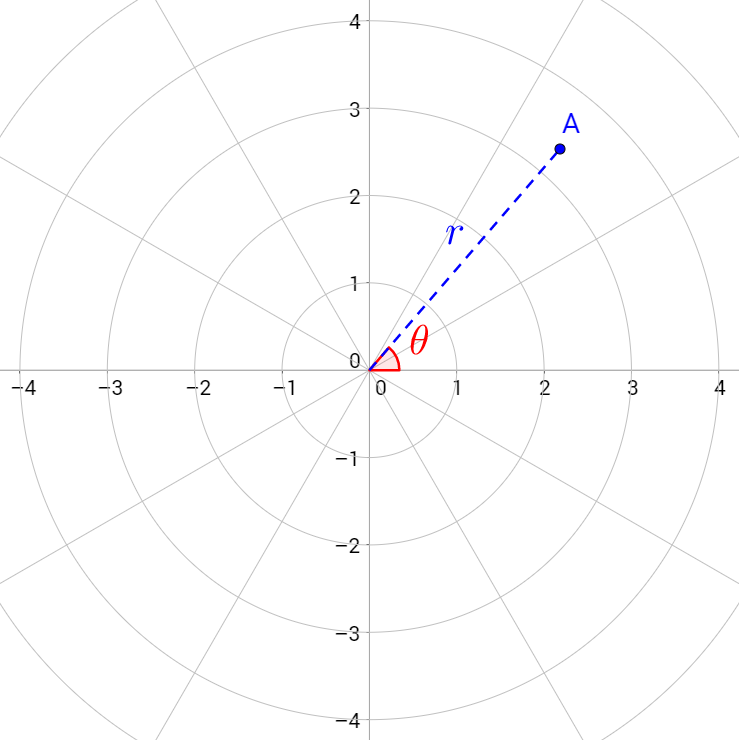
\includegraphics[scale=0.3]{sources/random_points_in_circle/images/polar-coordinate}
	\caption{Generation of a random point in polar coordinates given a random angle $\theta$ and a random radius $r$.}
\end{figure}

Despite its simplicity this approach is wrong as it does not produce points distributed uniformly in the circle. Before having a quick look at the mathematical proof it is instructive to have a look Figure \ref{fig:random_points_in_cirle:buggy} which is drawing a large number of points on the circle generated using this buggy solution. As you can see the points are not generated uniformly as their density is higher towards the center. 
The bottom line is, do not use this solution in an interview. A possible matlab implementation of this buggy approach is shown in Listing \ref{list:random_points_in_circle:buggy}.

\lstinputlisting[language=Matlab, caption=Non-uniform random point in a circle generation using Matlab,label=list:random_points_in_circle:buggy]{sources/random_points_in_circle/buggy_random_point.m}

\begin{figure}
	\label{fig:random_points_in_cirle:buggy}
	\centering
	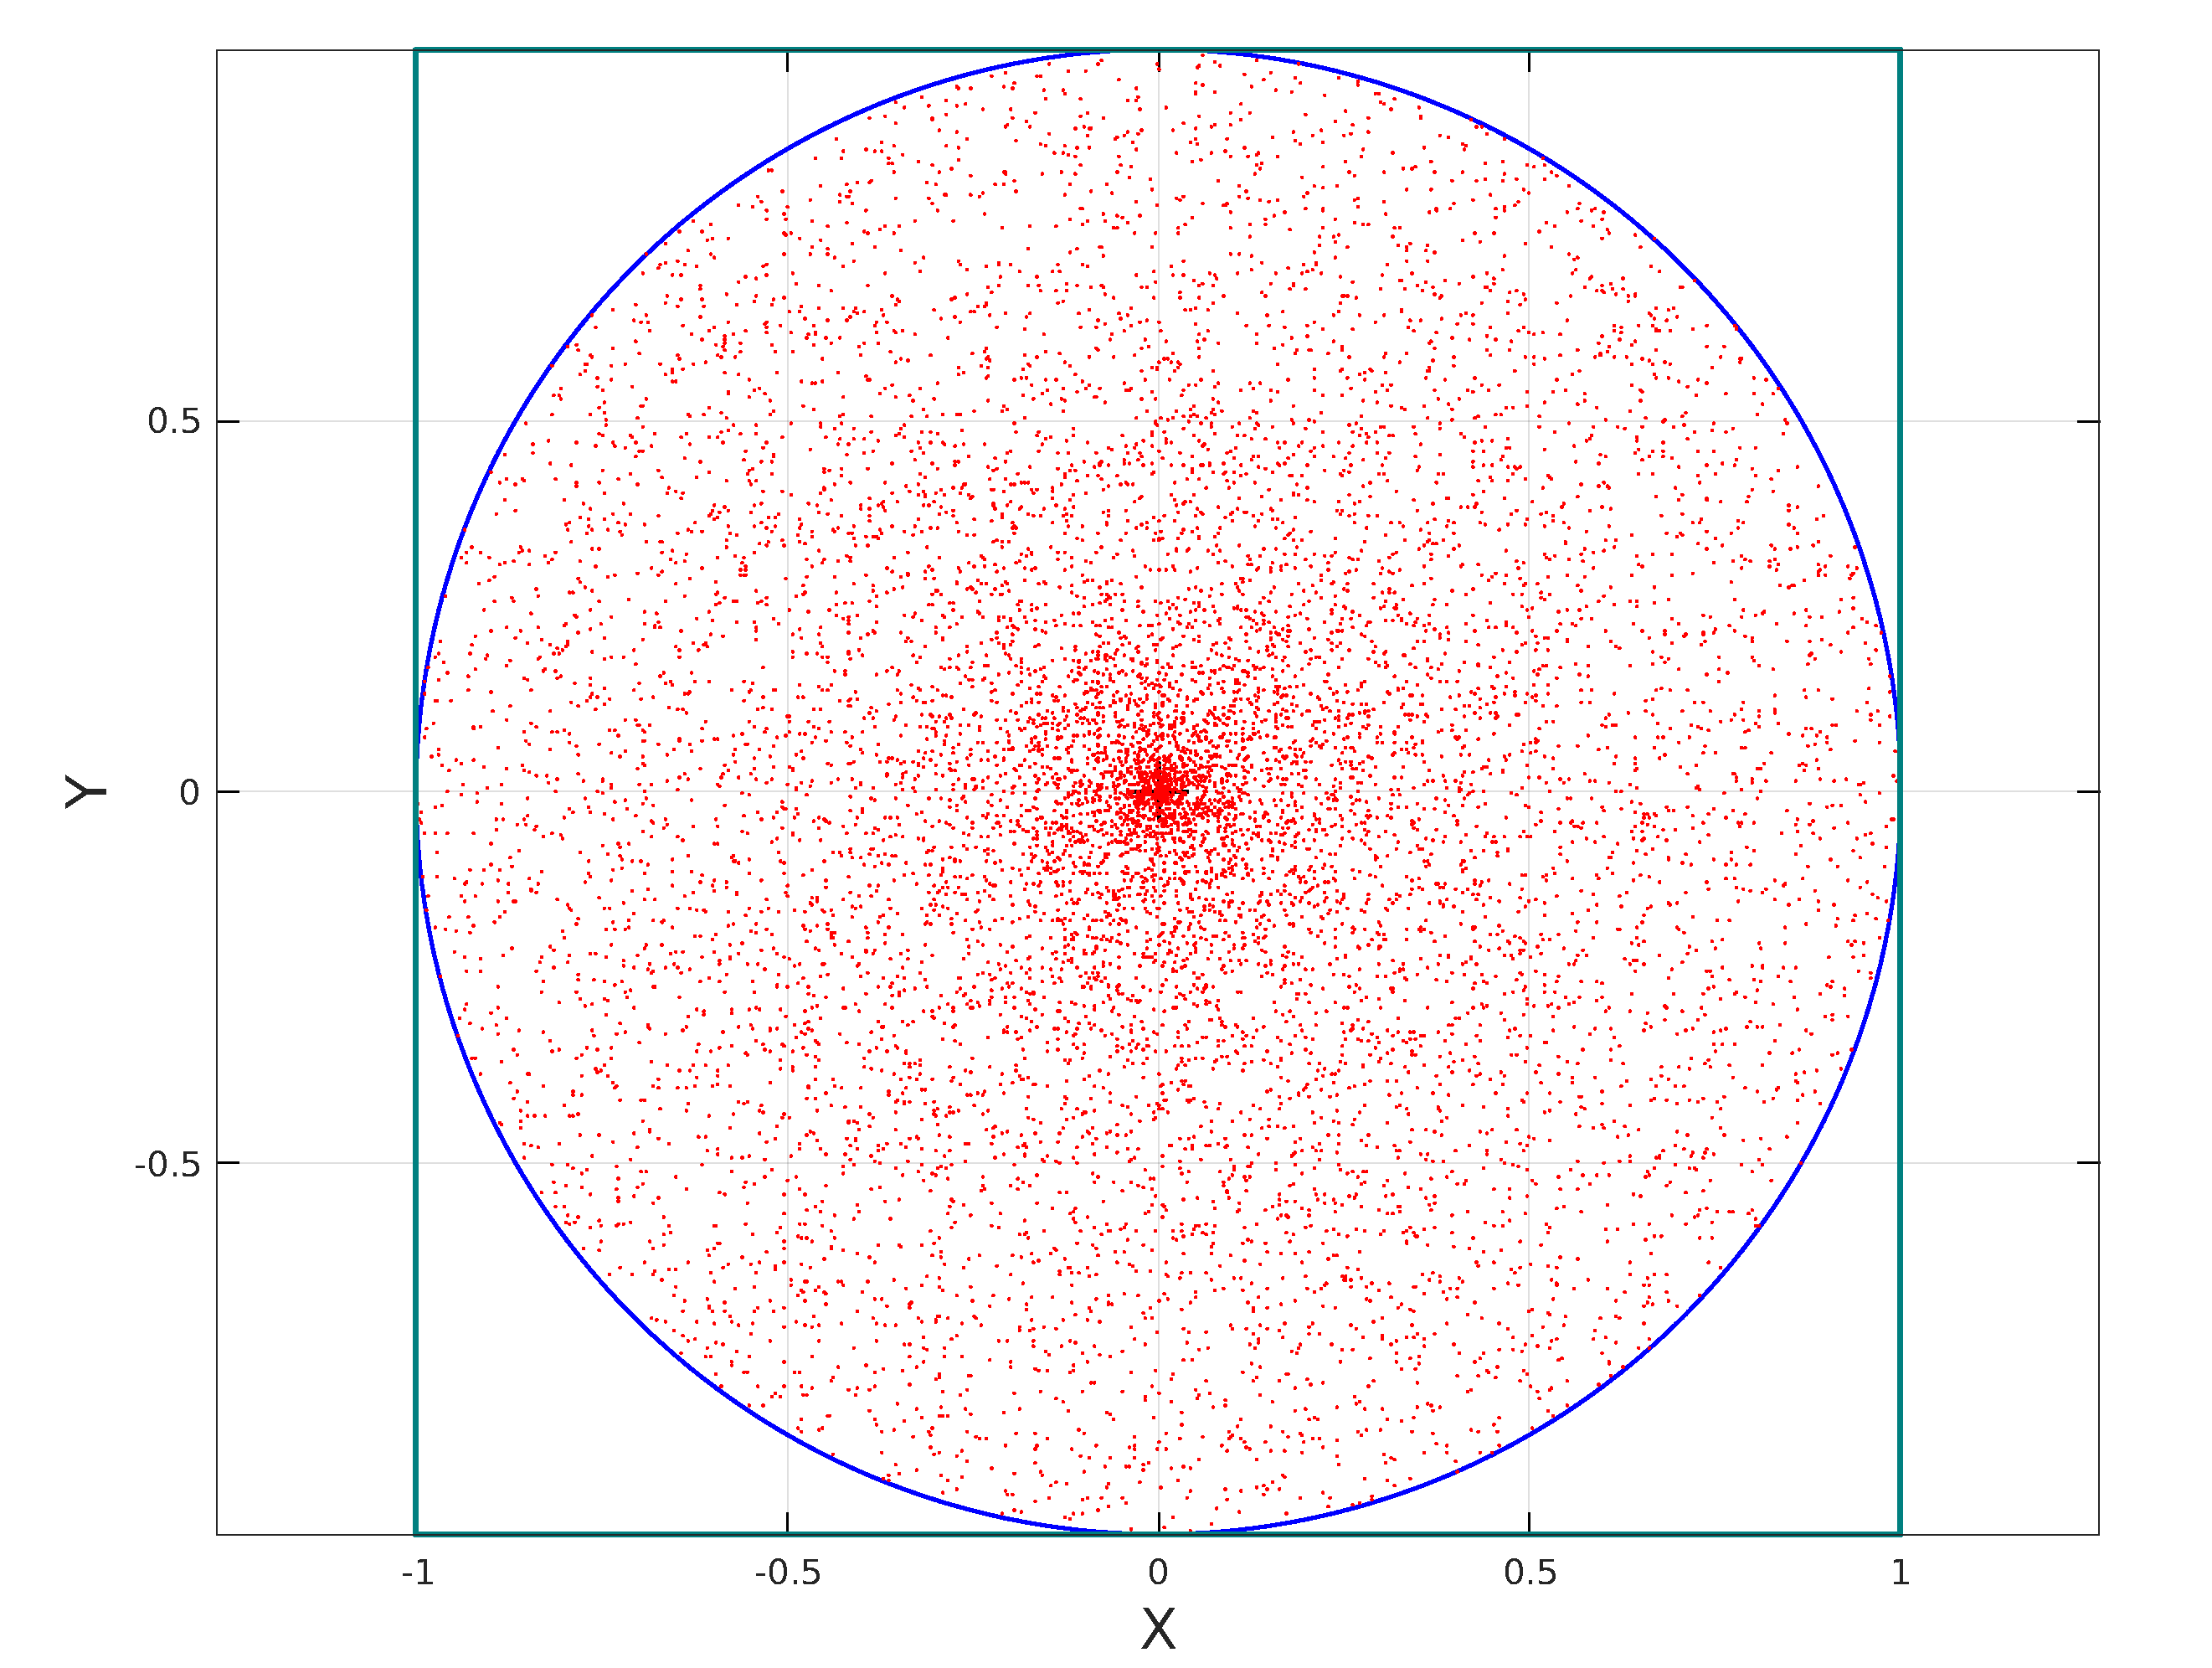
\includegraphics[scale=0.3]{sources/random_points_in_circle/images/buggy_points}
	\caption{Large number of points generated using the approach described in Section \ref{random_points_in_circle:sec:buggy}. Note that the density of points is not uniform as more points are packed around the center.}
\end{figure}

\subsection{Loop approach}
\label{random_points_in_circle:sec:loop}
A good way to make sure that the point density is uniform everywhere on the surface of the circle is to pick a point randomly in an enclosing square and making sure that we discard all the points that lie outside the circle. In other words, we keep asking for a random point $(p_x=\text{rand()}, p_y=\text{rand()})$ in the enclosing square until the following is true: $p_x^2 + p_y^2 \leq r$. This way we are guaranteed to generate uniformly distributed points because we pick those points from a set of points that are already uniformly distributed in a square, and we exclude those which are not inside the circle. This method is also known as exclusion method. Figure \ref{fig:random_points_in_cirle:loop} depicts a large number of points generate with this method.

The downside of this method is that we might need to generate a number of points in the square before getting lucky and picking one lying in the circle. We need to make on average $\approx 1.2732$ tries before getting a point in the circle. This number is  the ratio between the are of enclosing square and the area of the enclosed circle i.e. $\frac{(2r)^2}{\pi r^2} = \frac{4}{\pi}$. 

\begin{figure}
	\label{fig:random_points_in_cirle:loop}
	\centering
	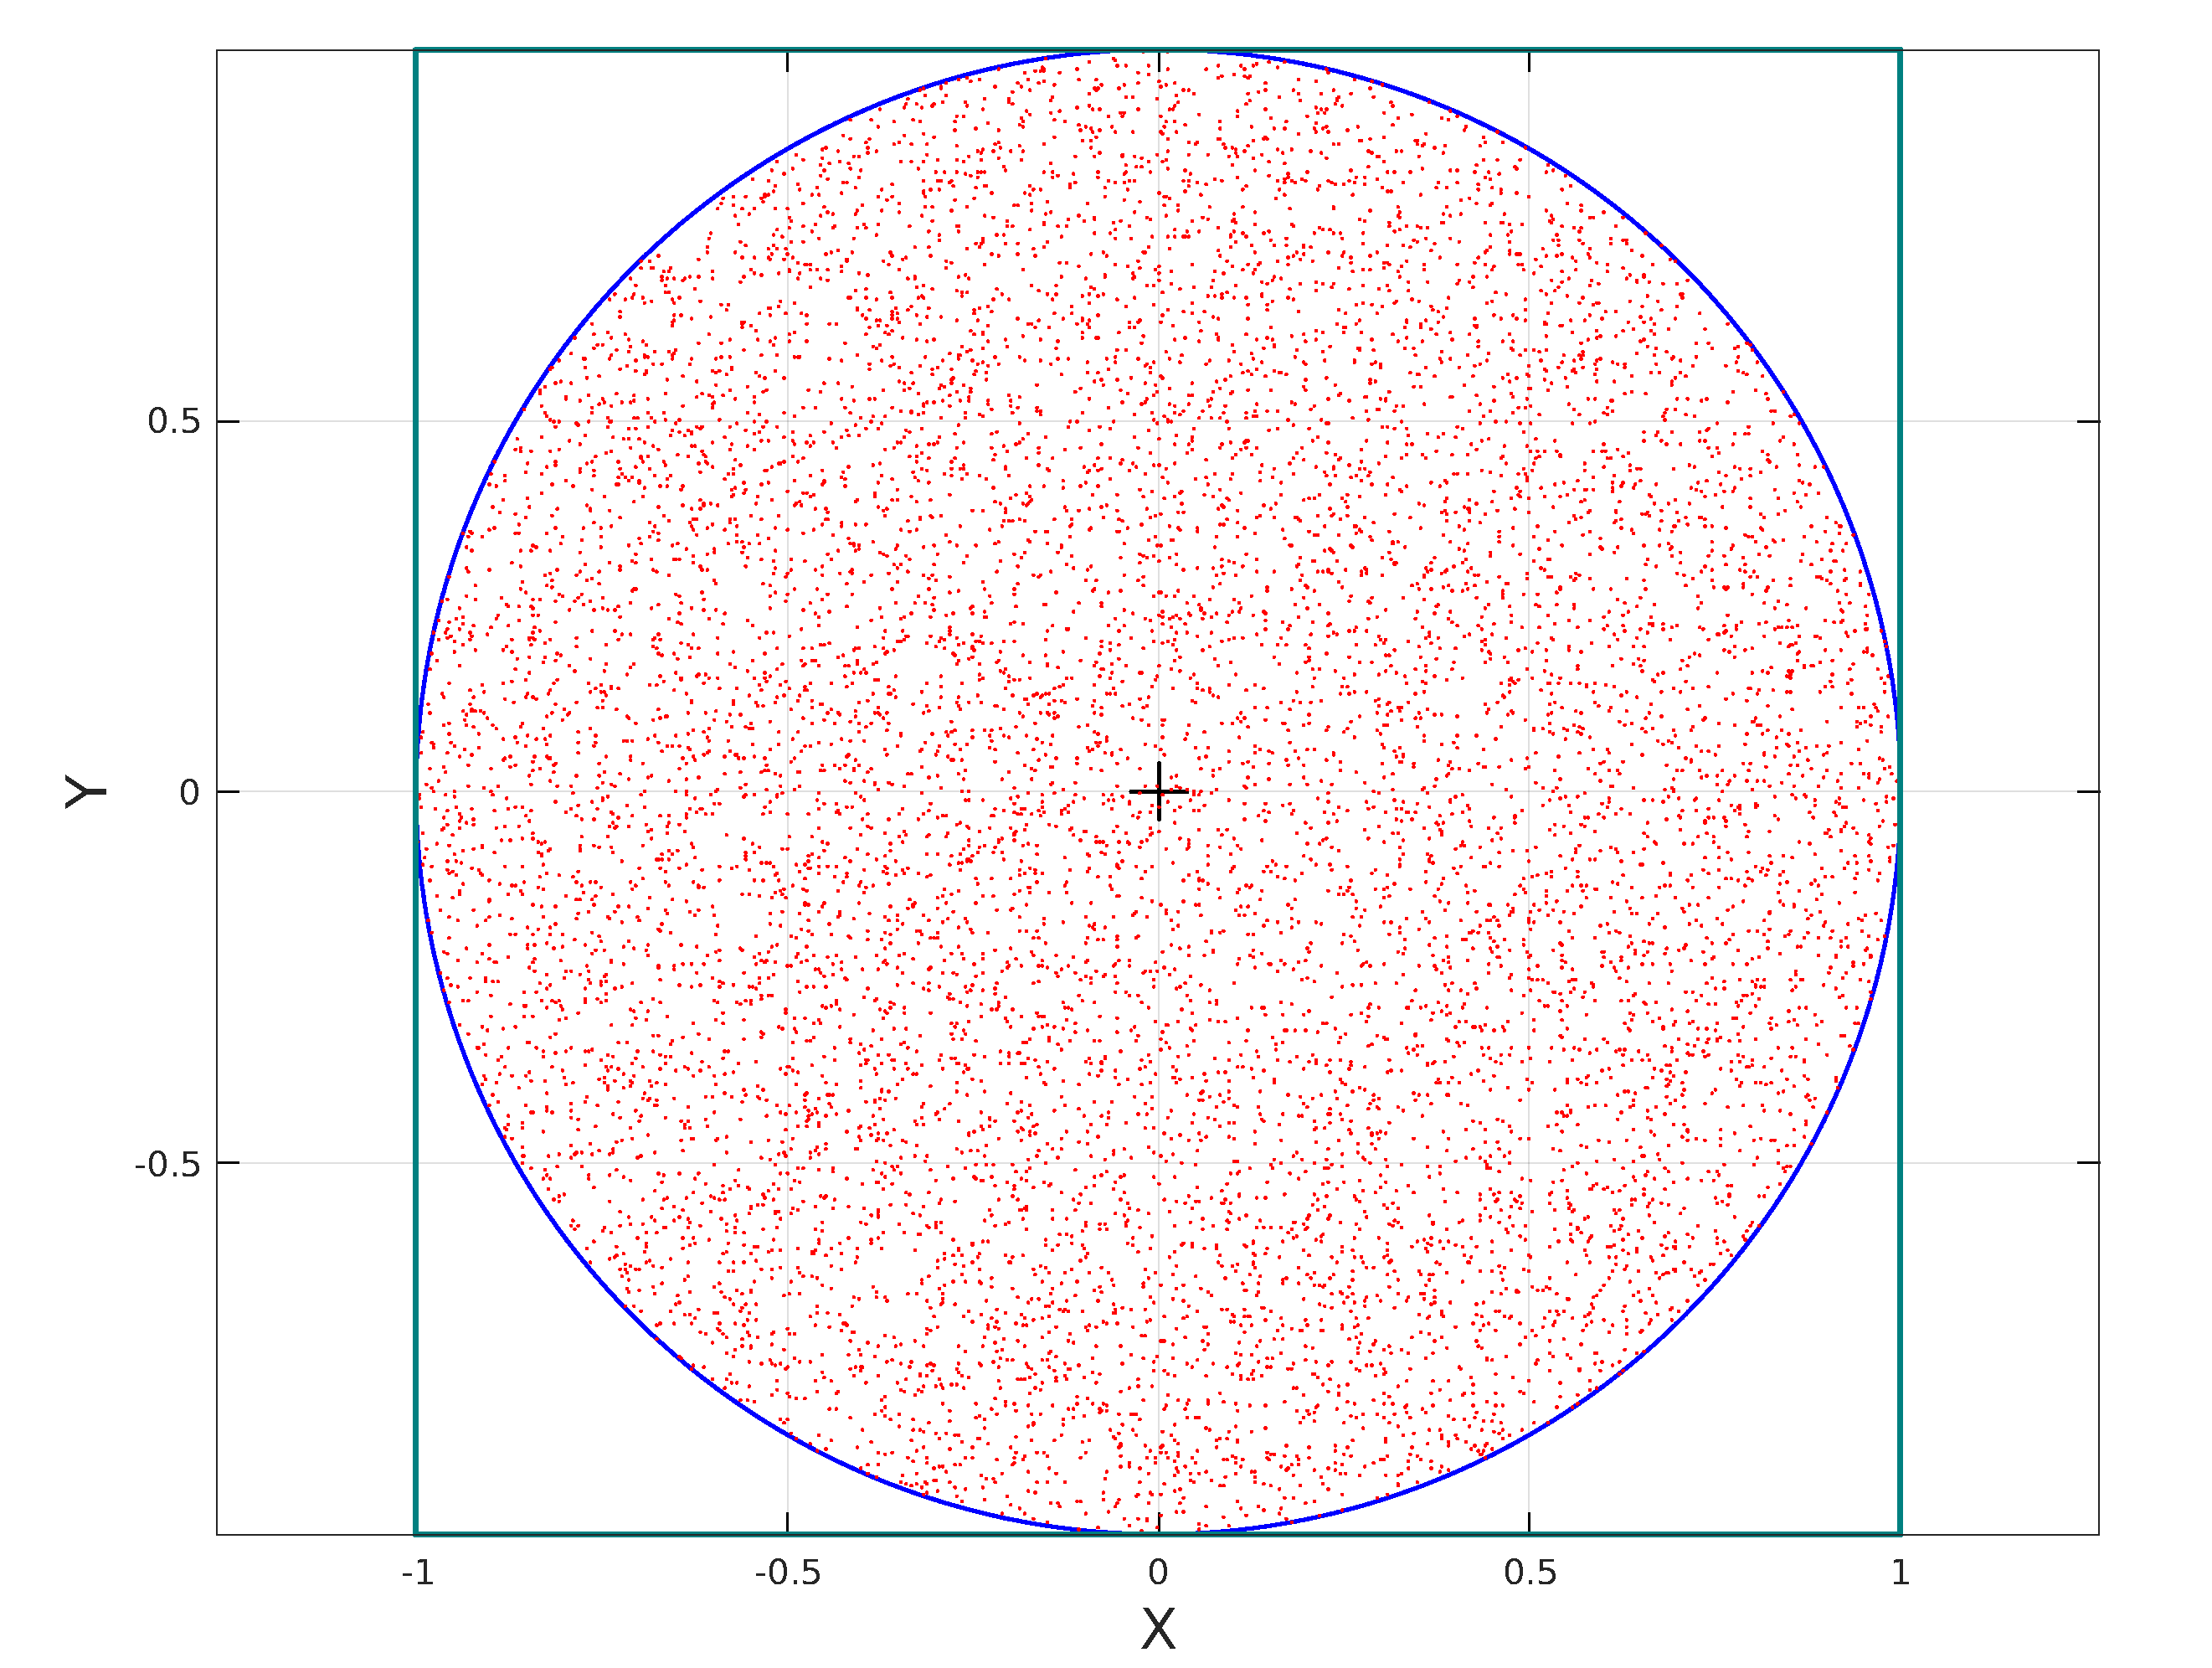
\includegraphics[scale=0.3]{sources/random_points_in_circle/images/loop_points}
	\caption{Large number of points generated using the approach described in Section \ref{random_points_in_circle:sec:loop}.}
\end{figure}

A Matlab implementation of this approach is shown in Listing \ref{list:random_points_in_circle:loop}.

\lstinputlisting[language=Matlab, caption=Random point in a circle generation using the exclusion method.,label=list:random_points_in_circle:loop]{sources/random_points_in_circle/random_point_loop.m}

\subsection{Polar Coordinates - The right approach}
\label{random_points_in_circle:sec:polar_sqrt}


In order for the points to be distributed uniformly it has to be that the average distance between the points has to be the same regardless of how far they lie from the center of the circle. This means that looking at the points generated on a circumference of radius $2$ there has to be twice as many points as the the number of points on a circumference of radius $1$. Twice as long circumference translates to twice as many points needed to maintain the same density. 
Another intuitive way  of looking at why simply picking a random angle and a random radius is not enough would be to think about having to distribute $10$ points at random on a circle of radius $1$ and $2$. It is clear that the circumference of radius $2$ would look emptier than the one with radius $1$ simply because there is more circumference to be filled but a constant amount of points. 

The fundamental problem with the approch described in Section \ref{random_points_in_circle:sec:buggy} is that the are of the circle is not uniformly covered. The random radius cuts through the area of the circle and this is the only parameter that affect how the points are going to be distributed across the area of the circle. Therefore we want to focus our attention to  how we can  pick a better radius by making sure that larger radii are picked more often to accommodate for the larger area they define. In other words, we need to ensure that our random function for the radius picking takes into account the area of our circle. 

Consider the area $A$ of a circle of radius $r$ i.e.  $A = \pi r^2$. We can rearrange the formula so that $r = \sqrt{\frac{A}{\pi}}$. What this formula is really telling us is that the radius is proportial to $\sqrt{A}$. We have a way of choosing the radius that depends on the area of the circle now. We can simply pick a random area at  random and then calculate the radius accordingly. This will make sure that the radius is picked taking into consideration the area of the circle. Figure \ref{fig:random_points_in_cirle:polar_sqrt} shows many points generate using this method. As you can see the points are generate uniformly across the area of the circle and the picture looks similar to Figure \ref{fig:random_points_in_cirle:loop}.

A C++ implementation of this method is shown in Listing \ref{list:random_points_in_circle:sqrtcpp}. Details on the random number generation in Modern \CC can be found in \cite{cit::std::random}.

\lstinputlisting[language=c++, caption=\CC implementation of the function for generating a random point in a circle described in Section \ref{random_points_in_circle:sec:polar_sqrt},label=list:random_points_in_circle:sqrtcpp]{sources/random_points_in_circle/random_points_in_circle_solution1.cpp}

\begin{figure}
	\label{fig:random_points_in_cirle:polar_sqrt}
	\centering
	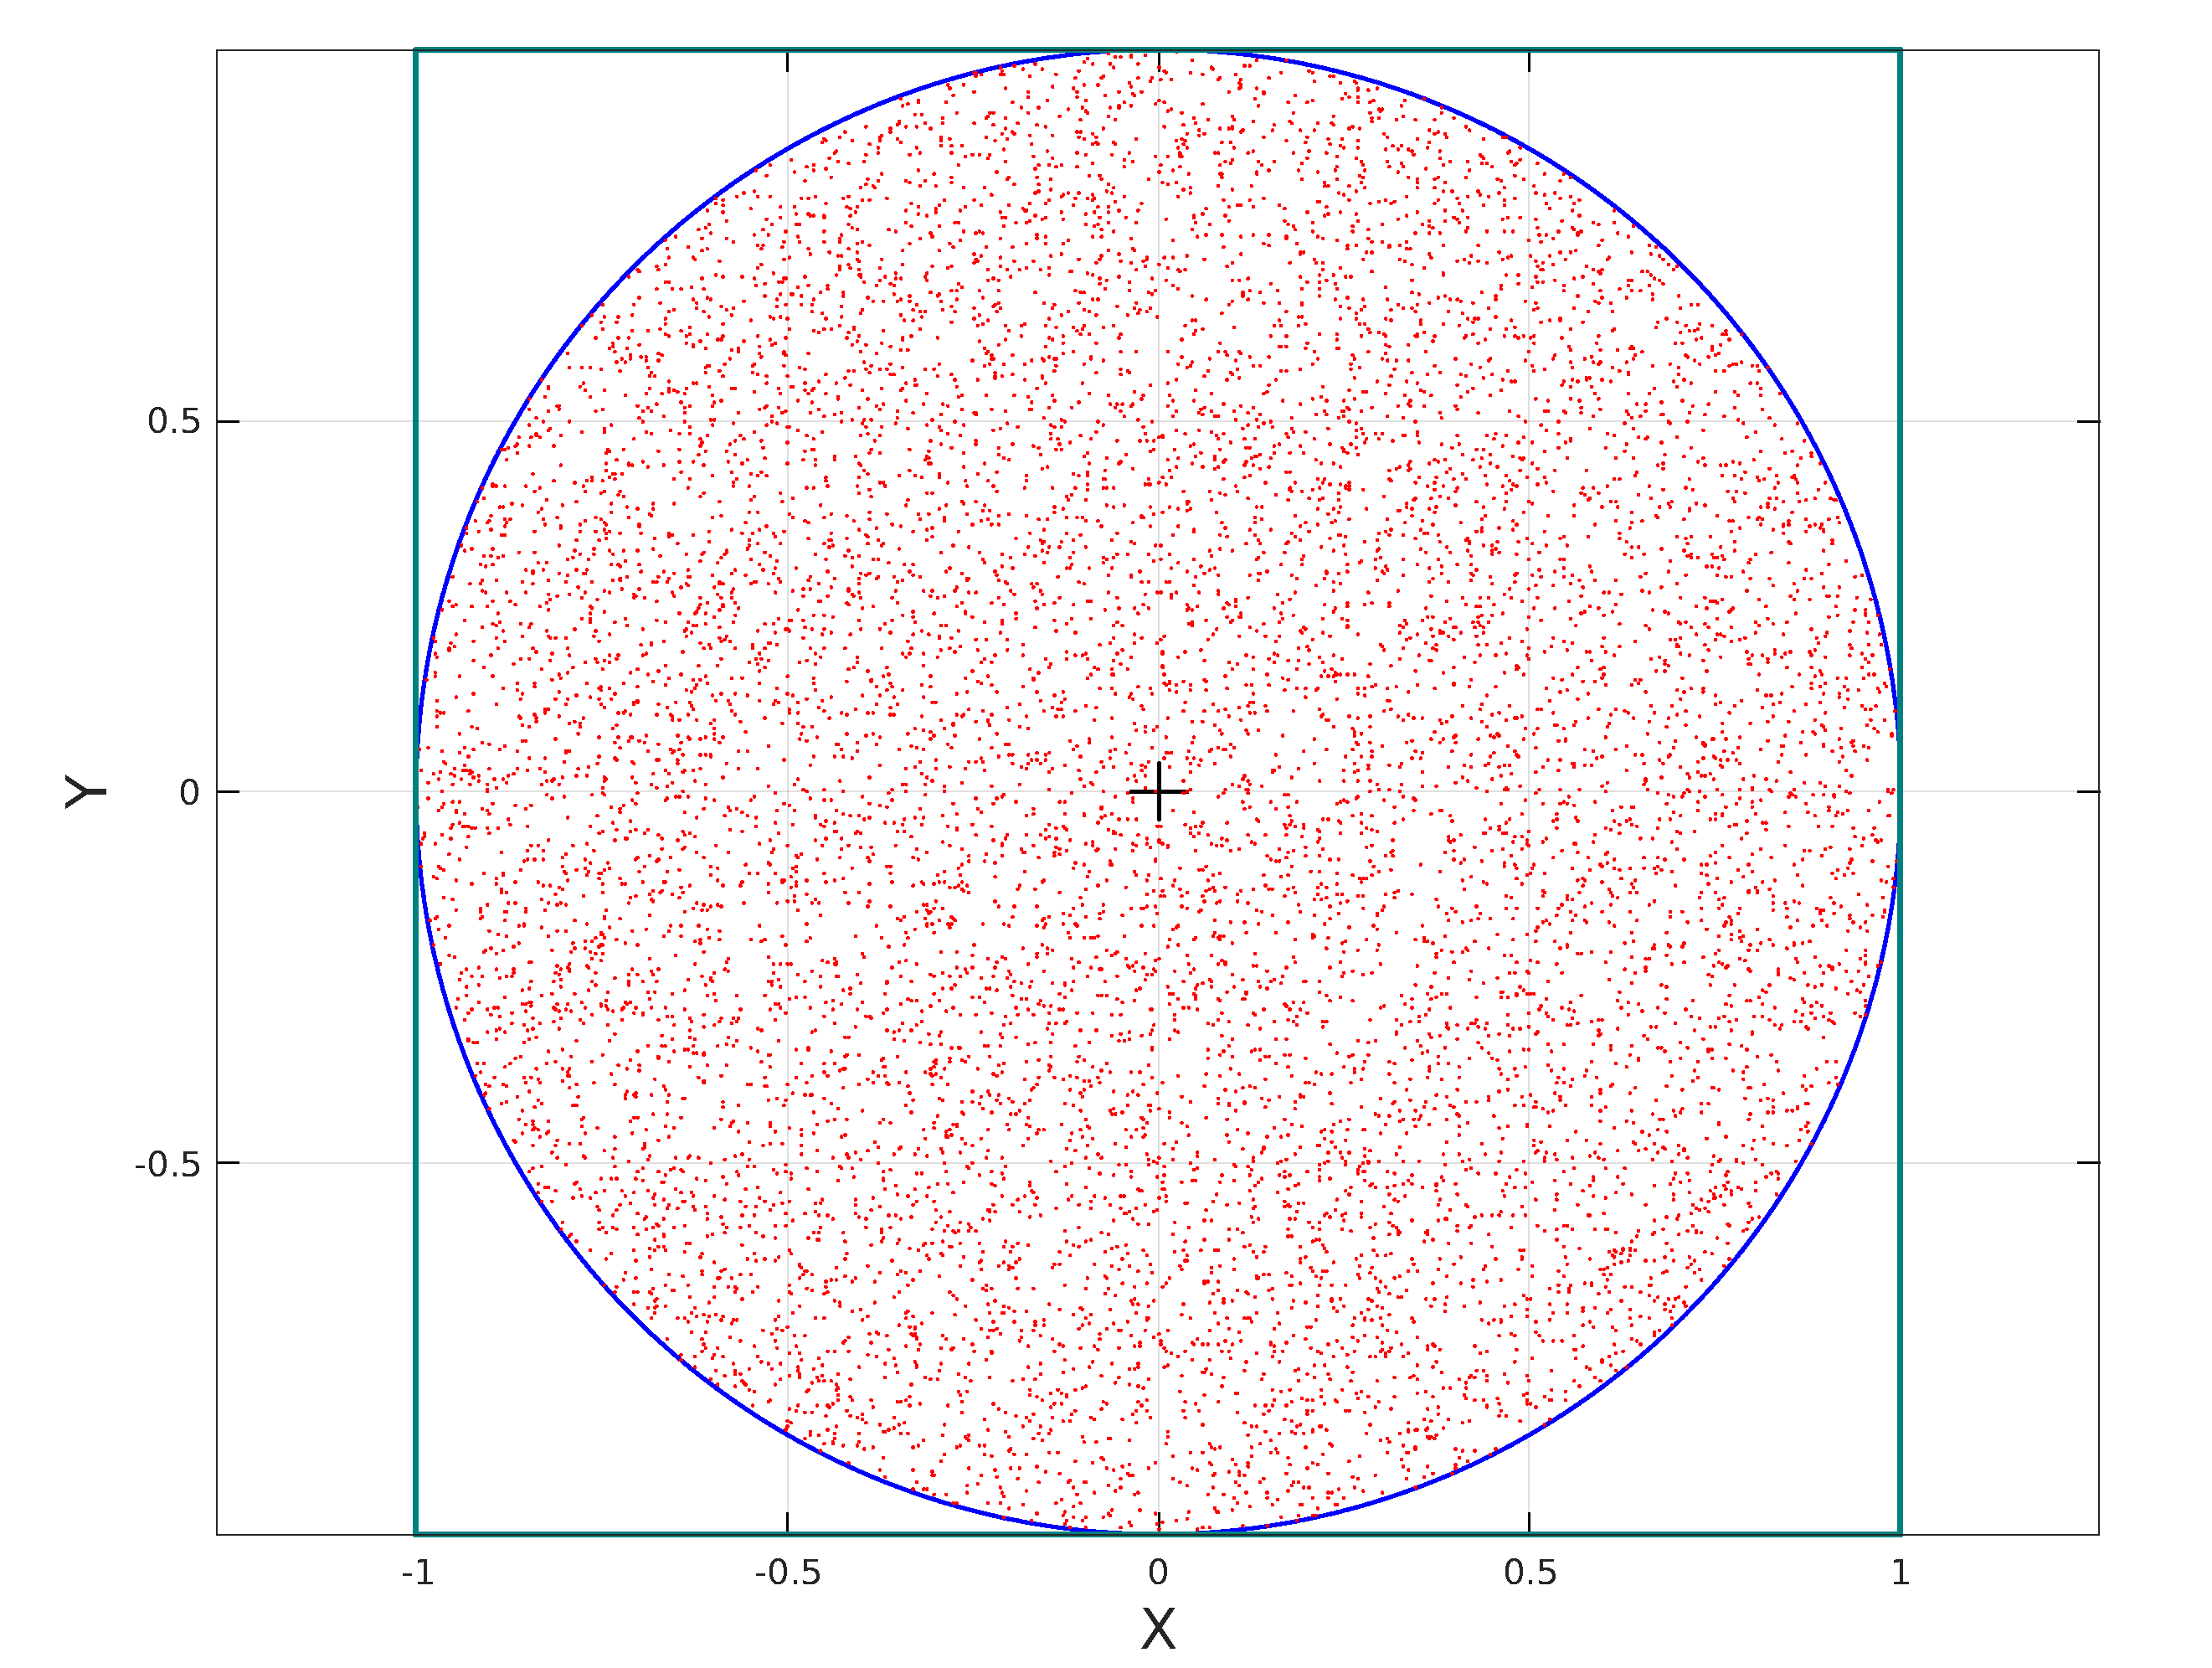
\includegraphics[scale=0.3]{sources/random_points_in_circle/images/sqrt_points}
	\caption{Large number of points generated using the approach described in Section \ref{random_points_in_circle:sec:polar_sqrt}.}
\end{figure}

A Matlab implementation of this approach is shown in Listing \ref{list:random_points_in_circle:sqrt}.

\lstinputlisting[language=Matlab, caption=Random point in a circle generation using polar coordinates and the $\approx \sqrt{A}$ dependency of the radius on the area of the circle.,label=list:random_points_in_circle:sqrt]{sources/random_points_in_circle/random_sqrt_area.m}

\subsection{Conclusion}
We looked into three two viable methods for generating random points withing a circle. The time and space complexity for all the two methods is constant even if the one presented in Section \ref{random_points_in_circle:sec:polar_sqrt} would most likely have better performances when included in an hot path i.e. in a loop for the generation of many random points.

All the code used to generate the Figures in this chapter is shown in Listing \ref{list:random_points_in_circle:drivercode}.


\lstinputlisting[language=Matlab, caption=Matlab driver code for the generation of all figures in Chapter \ref{ch:random_points_in_circle},label=list:random_points_in_circle:drivercode]{sources/random_points_in_circle/draw_points.m}
